\tikzstyle{env} = [rectangle, rounded corners, text centered, draw=black, fill=red!30]
\tikzstyle{vert} = [rectangle, rounded corners, minimum width=3cm, minimum height=1cm, text centered, draw=black, fill=blue!30]

\section{The Original Choice of ns3}
\label{ns3decision}
As the premier free and open source network simulation tool, ns3 seemed like the perfect choice for the project. The vast body of functionality that ns3 has built up over its lifetime means that most of the code that would be required could be reused, both shortening development time and reducing implementation errors.

Compared to its competitors, ns3 had the richest feature set, as well as the best API documentation. For this reason it appeared to be the easiest product to use.

\section{Why ns3 was Dropped in Favour of a Bespoke Solution}
Unfortunately, despite the promising findings of our preliminary research, it became apparent when ns3  was used to inform our initial design work that it would not be suitable for the project. The sheer amount of features in ns3 lead to a level of complexity which made it inaccessible. Whilst individual features were well documented and easy to use, amalgamations of these features were much harder to implement (not helped by a lack of documentation).

After some time spent struggling to actuate what were fairly simple tasks in the grand scheme of the project, it became clear that an alternative would need to be found. Given that even the masters level module at Warwick stops short of requiring students to perform more than simple tasks, the project would need something more accessible in order to achieve the requirement of being easy to use.

The research presented in section \ref{simSoft} shows the other network simulators that were investigated. Eventually, it was determined that there was no existing product which suited our needs to a high enough degree, and that creating our own simulator was the best option available. Of course, such a decision brought its own set of problems - primarily that a number of different algorithms and protocols would need to be implemented specifically for the application that was created (instead of being reused). Ultimately these drawbacks were outweighed by the ease of use that a domain specific application would bring.

Finally, a key advantage of creating a new simulator was that it would allow for easier deployment of programs to actual hardware. Given the breadth of drone models and software available, adapting an existing solution to be generic enough to interface with even a small subset of hardware available would have been a gargantuan task.

\emph{This section will focus on an analysis of the implementation of the simulator, more specifically on how each element of the simulator interacts and the general structure of the simulator itself}

\section{Code Structure and Development Methodology}
	The simulator was created to be as modular as possible with each subsystem having very clearly defined
	links to the other parts of the simulator. (for instance the methods of ``commMod" that interact
	with environment) Using this design allows for far easier modification and testing of each part
	of the system, as each part presents a ``contract" with the other pieces; so long as that ``contract"
	remains unchanged, the other parts of the system should be able to continue working identically
	even if the other components are changed. This also has benefits to possible optimisations of the system
	as any optimisations, will be trivially intergratable so long as they do not violate this ``contract".

	The simulator is extensible. This is actually the key to the way that the simulator works: the point
	of the simulator is that users extend the classes provided to use the simulator. This also
	allows users to extend the simulator in order to alter the way that the simulator works. As it is,
	the simulator is devoid of any non-essential features, but this is by design, as the main problem
	identified with NS3, was feature bloat, causing
	the entire system to be unfocussed and thus more difficult to develop for than a more focussed system.

	Despite seemingly contradicting the first point of this section, the simulator is also interconnecting,
	every system is related in some way to the other systems, Drone works very similarly to Base Station
	(which is to be expected, they both extend Messageable), and the way that broadcasts work is very similar
	to the ability to push visualisation elements.

	Ultimately, the primary implementation decision was to use multiple threads, which was to ensure that
	the system could emulate many independent machines at once (the primary purpose of the system).
	Unfortunately, this does lead to inefficiencies on machines with a lower number of available threads as
	the overhead in switching to and from virtual threads of execution is expensive computationally.

\subsection{The Environment}
		The environment code is the central hub of the simulator, handling all of the administration
		of tasks being performed by the system. The environment contains all of the sample sensor
		data, and contains references to all of the messageable components of the simulation.

		The environment's thread is what can be seen as the ``main" thread of the system, this is the
		thread that handles the movement requirements of the drones as well as keeping track of the
		system's internal representation of time (which is independent of real time in that
		the internal time is a multiplier specified by the user of the total number of movement ticks
		that have elapsed since the beginning of the simulation).

		Another responsibility of the environment code is to handle the broadcasting of messages to
		the drones, in the implementation this is achieved relatively inefficiently, using a simple collision detection
		method to check whether every known messageable is in range or not, this could be a target
		for optimisation for further development of the simulator, as will be outlined in the optimisation
		section below.

\subsection{Communication Modules}
		Communications modules act as intermediaries between the messageables they are attached to and
		the environment of the simulator. In actual deployment, the communications modules can be seen as a system
		handling lower-level network tasks required by the messageable. The communications modules are implemented
		in such a way as to reduce the workload of a developer creating messageable code, allowing for separation
		of labour into networking development and the actual programs to be executed on the messageables.

		Because of this, the communications modules primarily interface with the environment, passing messages
		to attached messageables from the environment and messages from the messageable to the environment.

		In terms of the actual functionality built in to the ``CommMod" class that represents the communications
		modules, it does little but pass messages and call the environment's ``broadcast" method. This is because
		the communications modules are not defined by the simulator but rather the user, allowing for any user defined
		communication protocols to be used.

		The job of each communication module's thread is to run the supplied function until it terminates.

	\subsection{Messageables}
		``Messageable" is the superclass of all classes designed to be a destination for messages, in this case
		drones, base stations, and all of their subclasses created by the user. The primary function of the
		code in the ``Messageable" class is to contain the virtual methods to be overwritten by the user, as
		well as some utility functions to facilitate communication between the running function of the messageable
		and its communication module.

		Each messageable's thread runs the user's overwritten function in the final subclass of the messageable.

		\subsubsection{Drone}
			Drone is a subclass of Messageable. The changes made to messageable with drone are simple, introducing
			new functions to facilitate the movement of the drone, as well as various utility functions to query the
			status of the drone, most of these functions are never called in the simulator itself, but rather are
			designed to be called by user defined subclasses of drone in the override of the ``run" function.

			Functions like ``move" do not actually cause the drone to move, but rather queue a movement for the drone
			that is then executed by the environment thread when the drone's ``upkeep" function is called.

		\subsubsection{Base Station}
			The ``Base Station" class is very simple as, aside from a constructor change, it is just a type transformation
			over Messageable. This is mainly to simplify the experience for the end user as extending messageable to create
			a base station would be possible, but would have been confusing.

	\subsection{Visualisation}
		The visualisation system provided a large set of implementation challenges. Because of the multi-threaded nature
		of the simulator, different threads can push elements to be visualised at any point. These element pushes are mainly
		handled through several helper functions that each call an underlying element pushing function with preset arguments.
		This simplifies both the implementation and use of these functions. The issue with this method is that the element list
		can be polled to change at any time, even when the visualiser is in the middle of a drawing operation. Due to the way
		C++ iterators work, and the fact the list has elements removed periodically (due to the fact that these elements are removed when they
		have exceeded their ``lifespan"), this could cause iterators previously pointing to valid elements to become invalid.

		For example, the element list consists of four elements, a base station, two drones and a broadcast. One of the drones is
		deactivated and thus removed from the element list, however the draw thread was drawing the broadcast at that exact
		moment. Because an element before the currently active element was deleted, the pointer to the active element becomes
		invalid. This means that the pointer can no longer produce a valid element, causing a segfault as unassigned
		memory is accessed.

		The solution to this problem was to lock both the ``step" function and the ``draw" function behind the same mutex lock.
		Effectively, this makes the two functions mutually exclusive, allowing only one of the two functions to be running at any
		given time. This causes any changes to the list of elements to be done only when there are not any active pointers to the
		list.

		The window management system used in visualisation was GLFW3, a platform independent system chosen due to its flexible
		nature and the fact that it can handle multi-threaded applications more easily than GLUT.

\section{Implementing Communications Modules}
Communications modules are responsible for performing tasks at level three of the OSI model\cite{normiec} (the networking layer). Depending on the noise function used by the simulator, it is also possible to have communications modules perform tasks in layer two (such as collision detection and avoidance). Whilst the base class is a part of the simulator itself, the actual implementation of routing algorithms are part of a separate library in their own right. In this way, the communications library is intended to be distributed with \textbf{octoDrone} without being required as a constituent part.

\subsection{Structure of an Individual Module}
\subsubsection{Sending and Receiving Messages}
		
When a communications module wishes to transmit a message to other units it invokes the broadcast method exposed by the simulation environment. Messages that originate from the communication modules messageable collect in a queue, which must be checked at regular intervals. When there is a message that the environment determines should be delivered to the communications module, it is deposited in a similar queue. When the module has a message it needs to pass to its messageable, it stores it in a third queue.

In addition to asynchronous messaging, the project design also called for synchronous message passing. This is achieved by having a callback function in the messagable which can be invoked upon receipt of an urgent communication. It is left to the communication implementation to decide which messages are important to interrupt the normal operation of the messageable for.
		
\subsubsection{Intermediate Processing}
The virtual function \textit{comm\_function} is called when the communications module is started and is expected to return when the associated program is ready to terminate. It should be used to perform any intermediate and non-delivery driven processing such as routing or time based commands.
		
\subsection{Structure of a Collection of Modules}
	
In order to facilitate easy distribution and use, collections of communication implementations are combined into libraries. Given the small size of a communications modules source code (often tens of kilobytes) it might be tempting to statically link them to simulation executables. The problem with this approach, however, is that it precludes the very thing that prompted the creation of communications modules in the first place - modularity. As such, communications code is packaged into a shared library which simulator executables are then linked against dynamically at compile time. This reduces the size of produced executables and makes updating communications code possible without requiring simulations to be recompiled.

\subsection{Access to Other Simulation Elements}
		
The architecture of the simulator requires that communications modules are able to interact with the simulator environment (to dispatch messages), as well as with the messageable with which they are associated. Since it is impossible to have all of this information available when the communications module is instantiated (creating a messageable requires a reference to a communications module as well), it is necessary to set the messageable associated with a communications object at a later time (but before the simulation is started). Thus, the procedure for bootstrapping a simulation is broadly as follows:

\begin{enumerate}
	\item Load the sensor data
	\item Create a simulation environment referencing the sensor data
	\item Create a communications module referencing the environment
	\item Create a messageable referencing the environment and the communications module
	\item Add a reference to the messageable to the communications module
\end{enumerate}

How these references are used is covered in section \ref{int-sim}.

\subsection{Integration with the Simulator and other Programs}
\label{int-sim}
The communications module class makes use of the following functions from the simulator:

\begin{itemize}
\item \textit{broadcast}
\end{itemize}

Programs for drones and base stations can make use of the following functions from \textit{CommMod}:

\begin{itemize}
\item \textit{push\_in\_message}
\item \textit{push\_out\_message}
\item \textit{comm\_function} (to start the CommMod)
\item \textit{set\_messageable} (used when defining simulations)
\end{itemize}

\subsection{Provided Implementations}
\begin{figure}[H]
\centering
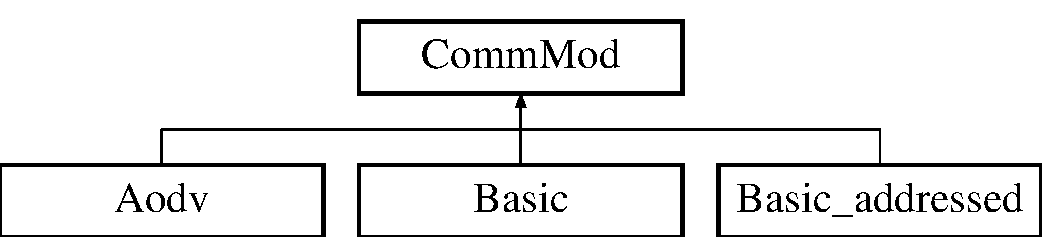
\includegraphics[width=\textwidth]{../documentation/latex/class_comm_mod}	
\caption{Inheritance diagram for the \textit{CommMod} class}
\end{figure}

\subsubsection{Basic Messaging}
\begin{figure}[H]
\centering
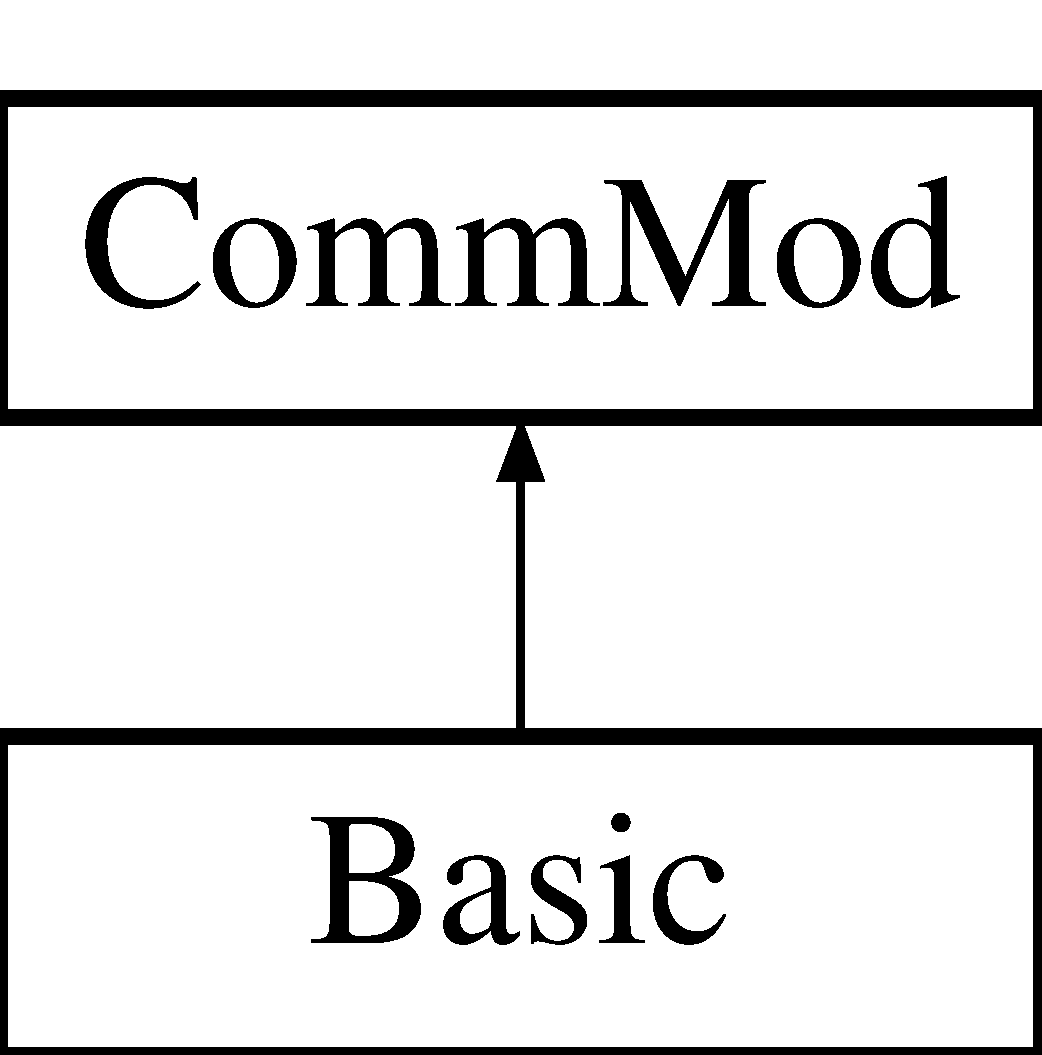
\includegraphics[scale=0.2]{../documentation/latex/class_basic}	
\caption{Inheritance diagram for the \textit{Basic} class}
\end{figure}

The basic messaging implementation provides the simplest possible way of sending and receiving messages. This can be useful when creating programs for messageable units, as it removes the need to consider routing problems, units being out of range, and a whole host of other potential issues. Additionally, it provides a good method for simulating existing programs which were not written with \textbf{octoDrone} in mind and may perform their own addressing. In this way it contributes to octoDrones ability to be generic and flexible. 

In this implementation, all messages that are sent are received by all nodes, regardless of range. Messages sent include payload information, but do not store information on the sender or receiver.
	
\subsubsection{Addressed Basic Messaging}
\begin{figure}[H]
\centering
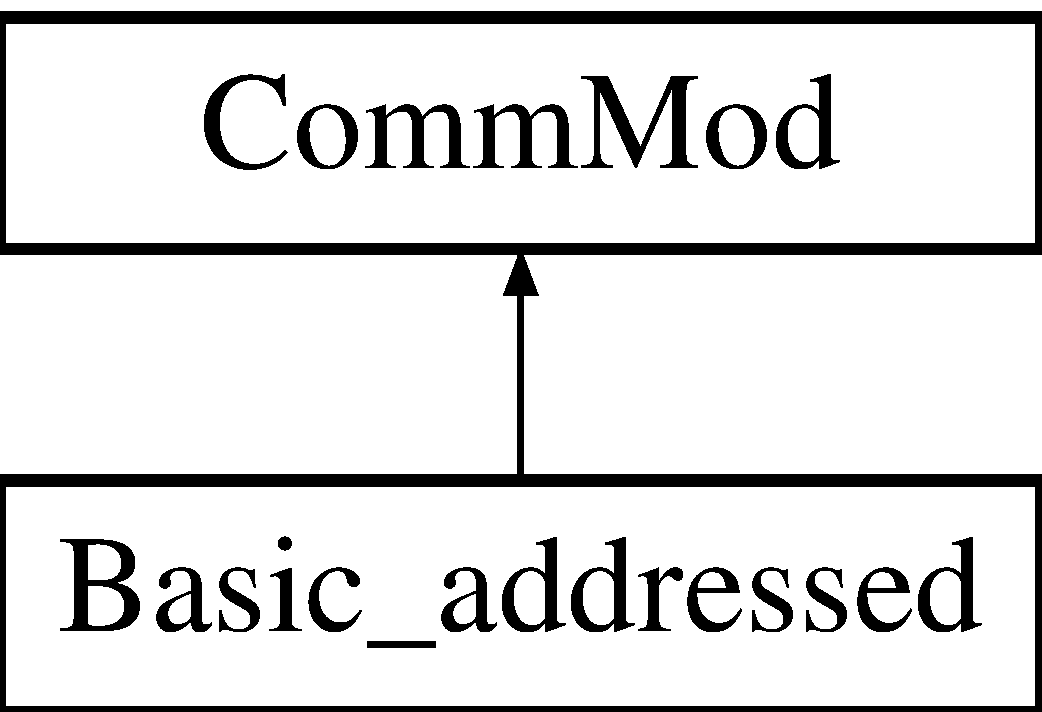
\includegraphics[scale=0.25]{../documentation/latex/class_basic__addressed}
\caption{Inheritance diagram for the \textit{Basic\_addressed} class}
\end{figure}

The addressed basic messaging implementation extends the above algorithm to additionally take into account the sender and intended recipient of a message when choosing which packets to deliver and which to drop. It is intended to be used for passing messages between programs and communication modules in a way which prevents the need to include code to serialise and deserialise addresses. If appropriate, it can also be used with external programs as described above.

In this implementation, all messages that are sent to an IP address are received by all nodes with that IP address, regardless of range. Messages include payload information as well as the IP addresses of the sender and intended recipient. Messages sent to the broadcast address 255.255.255.0 will be received by all nodes in the simulation.	
	
\subsubsection{Ad hoc On-Demand Distance Vector Routing}
\begin{figure}[H]
\centering	
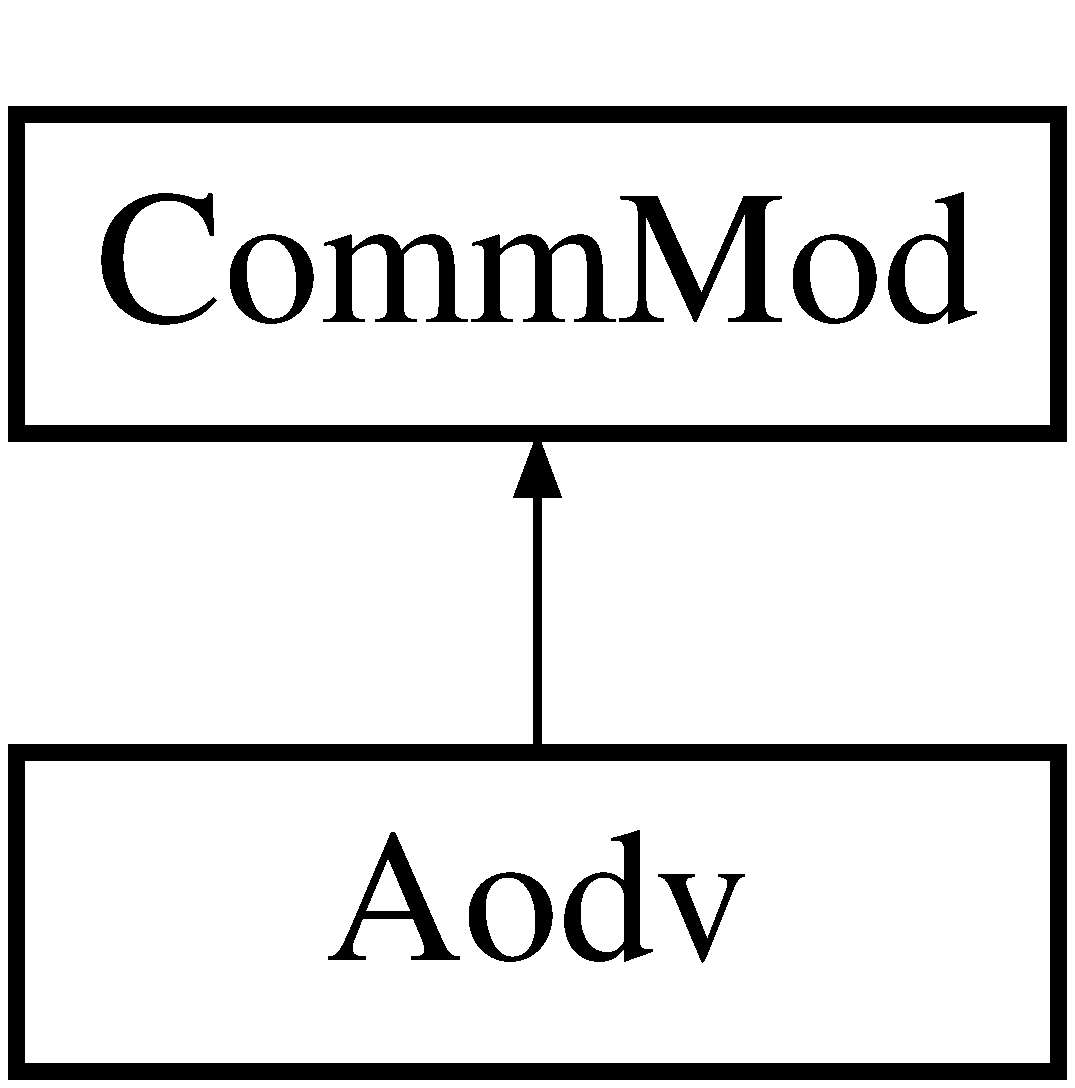
\includegraphics[scale=0.2]{../documentation/latex/class_aodv}	
\caption{Inheritance diagram for the \textit{Aodv} class}
\end{figure}

The Ad hoc On-Demand Distance Vector Routing (AODV) implementation provided in the communications library gives an example of how a more sophisticated routing algorithm can be used within the simulator framework. AODV is designed to be used in mobile ad hoc networks and offers loop free, just-in-time routing that is fault tolerant and capable of reacting to the movement of nodes.\\

\noindent\textbf{Overview}
\label{AODVdesc}

In order to explain what is happening under the hood of the AODV implementation provided with \textbf{octoDrone} it will be useful to first cover the basics of how the algorithm operates. A node A which wishes to send a data packet to node Z transmits a Route Request (RREQ) to its neighbours, which serves the dual purpose of notifying it of the next hop in the most efficient path to Z, but also of notifying the routes along the way where they should direct messages addressed to Z\cite{perkins2003}. If a unit receives a route request for which it does not have a valid route it broadcasts the route request to each of its neighbours in order to propagate the route discovery. 

When the RREQ is received by a node which has a route to Z, either because (as in this case) it \textit{is} node Z or because it is already part of a route to Z, that node creates and returns a Route Reply (RREP) packet. This packet is used by every node on the reverse route to store the next hop to the destination, Z, and is forwarded to the nodes that sent the RREQ. Incremented sequence numbers are used to make sure that information remains fresh as for loop prevention. 

Once the sending node, A, receives an RREP it can send out its data packets via the next hop on the route that was just discovered. This route will be cached for a period of time before a new discovery period must take place. If at any time there is an error during transmission, the node encountering the issue sends out a Route Error (RERR) packet to notify other nodes that cached routes using this hop should be invalidated.\\

\noindent\textbf{The Routing Table}
The AODV implementation has a special data structure to represent entries in an AODV routing table. As per the RFC (documents by the Internet Engineering Task Force containing technical and organizational notes about topics such as internet protocols), this contains the sequence number of the destination node, the time after which the route is no longer considered active, the hop count to the destination node, and the next hop on the route to the destination node. Each AODV communications module keeps a map of destination IP addresses to route objects, which is known as its routing table.\\

\noindent\textbf{Message Types}
\begin{figure}[H]
\centering	
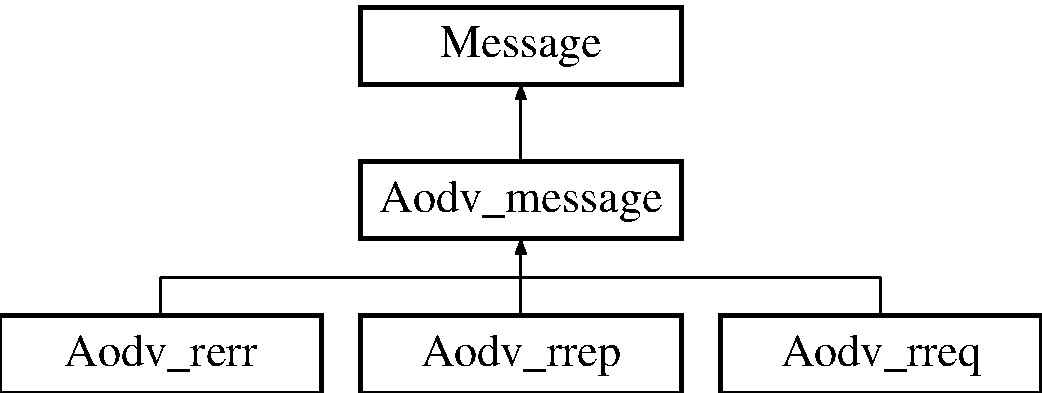
\includegraphics[scale=0.6]{../documentation/latex/class_aodv__message}	
\caption{Inheritance diagram for the \textit{Aodv\_message} class}
\label{aodvmess}
\end{figure}

In order to easily handle the different types of messages handled by AODV (RREQ, RREP, etc.), the implementation defines a basic AODV specific message class which contains the fields common to all AODV messages. This is then extended by individual classes in order to completely define which fields are required by each message type. This is shown in figure \ref{aodvmess}.\\

\noindent\textbf{Sending Messages}
With the above classes in mind, we turn to the question of how octoDrone goes about sending messages. Initially, messages which have been deposited into the outbound queue must be deserialised into a structure containing the message payload, the destination address of the message, and the source address of the message (in some situations this may be different from the address of the communications module). This happens because messages are always sent to and received from the environment in string form. While it may at first seem inconvenient, it is necessary in order to preserve the integrity of messages if they are sent over a network (which is the case if we are running a deployment on real hardware). After this the routing table is queried to find out if the node already has an active route to the destination. If it does, then a data packet is constructed immediately and dispatched via the next hop on the route to the destination.

If there does not exist a route in the cache, things become a little more complicated. Because the route discovery process requires that we send and receive a number of different packets before sending the message is considered done, we need to keep track of internal state. In octoDrone's implementation of AODV, this is done by keeping track of the current message we are sending, as well as the stage in the route discovery process we are currently at. This means that whenever something is triggered by a message being received, it can access this information (and update it if required), even when the original message object has long since gone out of scope. After the state information is created, a helper function is used to create the RREQ which will initiate the AODV protocol on other nodes. This is then sent using a call to the simulation environment. At this point there is nothing else to do but wait for messages to be received.\\

\noindent\textbf{Receiving Messages}
When a message is received, the communications module unwraps just enough of it to determine the type of message that has been delivered, which will be one of the AODV types, such as RREQ (this type is internal to AODV, and should not be confused with the type property of the base message class which is used to denote emergency packets). This information is then used to select an appropriate deserialisation function to apply to the message in order to transform it from a string into an AODV data type. Each of the types has its own processing method, which determines what action (if any) to take given the message contents and the internal state of the communications module.

For RREQ messages, the node checks to see if the message was a hello message (described in section \ref{hello}), and if so we determines if there is an active route to the sender (who will be one of its neighbours), and add a new route if it does not. A reply is sent to the sending node so that it can compile route information about other units in the network. If it is not the case that the message is a hello message, then it must be route discovery from another node. If the communications module has an active route to the destination mentioned in the RREQ, then a helper method is used to generate an RREQ packet to reply with. This is sent via a call to the simulation environment. Otherwise, the node's internal state is updated to record that it is participating in remote initiated route discovery, and the RREQ packet is forwarded after decrementing the time to live (TTL) field and incrementing the hop count. In order to keep the implementation small and simple, nodes do not respond to RREQ requests when they are part way through route discovery for themselves or another node.

When an RREP is received, the communication module first checks to see if the route it has to the sender (previous hop) is up to date, modifying the routing table if appropriate. Afterwards, it checks to see if the route was for itself (to send a data packet) or for another node (remote initiated route discovery). Multiple RREP packets for a single route indicate that there exists more than one possible path. In this case, the route with the lowest hop count is chosen (the reply window is defined by the path discovery time variable which is set at instantiation). If the former, then a data packet is constructed using the new routing information, and sent via a call to the simulation environment. Otherwise, the information is passed on (with a decremented TTL). Keeping track of hop counts is done by the helper function.

Upon receipt of an RERR packet, the communication module marks the route as invalid (achieved here by setting the active route timeout to zero), before broadcasting this information so that affected nodes can update their local routing tables.\\

\noindent\textbf{Broken Links}
But where do these RERR packets come from? It may be that a node receives a message for which it does not have a route. It may also occur that a node loses connectivity with one of its neighbours. If either of these scenarios come to pass then the receiving node will broadcast an RERR message to the node which precedes it in the route. Given that the octoDrone implementation of AODV only stores forward routes for simplicity, all RERR messages are sent upon message receipt instead of also being sent upon link failure. This makes sense: because octoDrone does not emulate the lower layers of the OSI model, nodes do not have access to information about link statuses. One way of mitigating this is to use hello packets as described below in section \ref{hello}. When a node fails to receive a hello packet for a neighbour which is listed as the next hop for one of the route in its routing table (this includes neighbours which are the next hop and destination for a route), it will mark that route as invalid and propagate an RERR the next time that route is used.

\subsection{Extension: Hello Messages}
\label{hello}
The RFC for AODV also mentions the use of hello messages as a means of broadcasting connectivity information. While the document suggests that nodes should only broadcast hello messages if they are part of an active route, to account for the differences mentioned above, all nodes using the octoDrone implementation of AODV will send hello packets on a regular basis.

\section{Summary}
The above sections have shown how the designs for octoDrone communications have been implemented, covering the structure of communication modules, message types, and how these components integraye with the rest of the software. In the next chapter these concepts will be taken one step further with the jump to real hardware instead of simulated hardware as was discussed here.

\section{Potential Optimisations}
	This section will highlight several areas for optimisation, how they are inefficient and why they were implemented this way.
	The first and most obvious area for optimisation is in the environment code, specifically the way that broadcasting works. As the
	code currently exists, when a broadcast occurs, the entire list of messageables is tested, each one being checked whether it is
	within the range of the broadcast. If it is then the message is sent to that messageable. A potential optimisation 
	(especially for broadcast-heavy programs running on the simulator) would be to limit the messageables that receive the
	message to those in the general area of the broadcast perhaps through some kind of segmentation of the environment space in to
	a three dimensional grid which contain a subset of all elements.

	Another area to be optimised could be the main threads calling of the upkeep functions on the drones The way it works
	in the provided implementation is that environment calls upkeep one drone at a time. This works fine, but there are no dependencies
	between each drone's upkeep method, so parallelising this process could improve performance, it does however cause the 
	creation of even more threads (which this system already creates a lot of), so this optimisation could only be valid for
	systems that can afford to have a large number of threads running at once.

	These are the obvious algorithmic optimisations that could be done, also to be considered could be reducing the amount of threads
	that the system creates in order to improve performance on machines with fewer hardware threads (as switching the thread
	of execution can be expensive).

\section{Review Against Original Objectives}
	The only objective that pertains to this section is ``Implement a network simulator" which requires analysis as to whether
	the implemented system fulfills this objective. The objective requires a system that is capable of supporting the creation 
	of a network of drones which are capable of sending messages and reacting to messages they recieve. Due to the way that the
	system works, this requirement is fulfiled, arbirtary drone programs can be implemented through user defined Drone, CommMod, and
	BaseStation subclasses.

	However, this objective also requires ``Specifically tailored to our domain". This is where the analysis is required as
	the domain in which the project lies is flexible. In order to fulfil this objective the system would have to enable the
	creation of drone programs that can perform arbitrary tasks. The system fulfils this requrement too: the system was crafted
	specifically with this in mind, the simulator specifies very little, causing no bottlenecks or restrictions (with the exception
	of requiring exactly one base station).

\section{User Manual}
	In order to use the simulator, users must extend BaseStation once implementing the run and message\_callback methods and pass it to an
	instance of Environment created with the sample data for the simulation. From here, the user must implement extensions to Drone and CommMod,
	one for each type of drone and communications module required. Many projects will require only one of each of these, but it is
	possible that a project with multiple types of drones could be created. Instances of the created drones should be passed to
	the environment instance. In the run method for any Drone or BaseStation derived class, a user can use the ``send\_message" method
	in order to send a message to the communications module for broadcasting, the ``wait\_for\_message" method in order to wait for
	the next incoming message (implementing the ``message\_callback" function allows for non-blocking communication), and use the
	``get\_time" and ``get\_position" methods to get the time and position respectively. Drone adds the functions ``move", ``turn",
	``getMaxSpeed", ``getSpeed", ``getAngle" and ``hasFinishedMoving" which return their respective values or perform their respective tasks. The
	function ``sense" allows the drone to gather data of the supplied type, emulating the use of different sensors with different strings supplied to the
	function.

	The ``CommMod" extensions allow the use of the ``broadcast" method as well as the ``pass\_message" method, with these sending
	messages into the environment and to the attached messageable respectively. The function of ``comm\_function" which should be
	extended by every extension of CommMod is the actual communication module code.

	The purpose of the simulator is to simulate the physical deployment of code on drones. The idea is that with a properly
	configured drone or base station, a user can take the code in the simulator and run it on physical drones and base stations
	with, no work to port the code to the new machine. See the physical deployment section to see an example of this.
